\documentclass[tikz,border=6pt]{standalone}
\usepackage{tikz}
\usetikzlibrary{arrows.meta,positioning}

\begin{document}
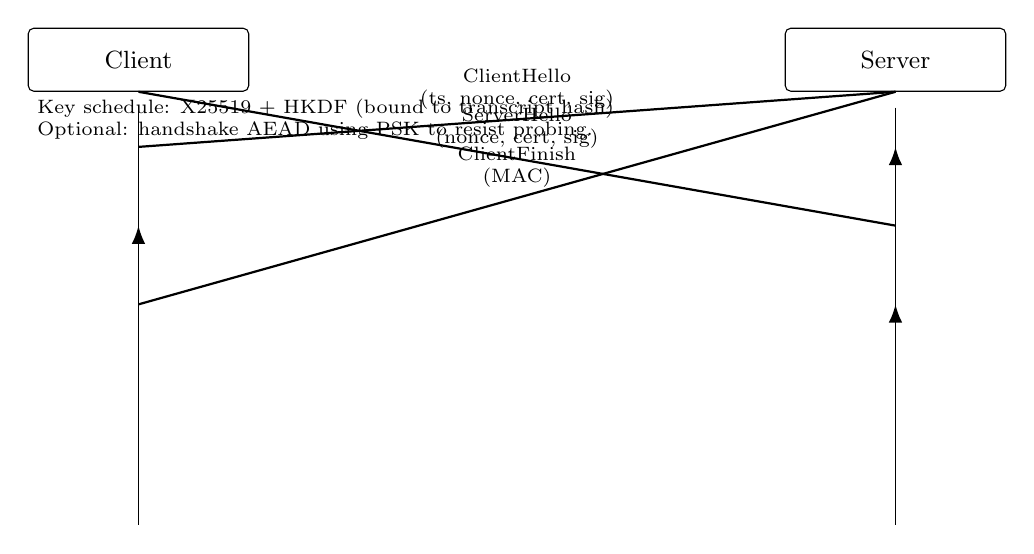
\begin{tikzpicture}[
  font=\small,
  lifeline/.style={draw,rounded corners=2pt,minimum width=2.8cm,minimum height=0.8cm,align=center},
  msg/.style={-Latex,thick},
  note/.style={align=left,font=\scriptsize},
]
  \node[lifeline] (c) {Client};
  \node[lifeline,right=6.8cm of c] (s) {Server};

  \draw (c.south) ++(0,-0.2) -- ++(0,-5.3);
  \draw (s.south) ++(0,-0.2) -- ++(0,-5.3);

  \draw[msg] (c.south) ++(0,-0.7) -- node[above,align=center,font=\scriptsize]{ClientHello\\(ts, nonce, cert, sig)} (s.south) ++(0,-0.7);
  \draw[msg] (s.south) ++(0,-1.7) -- node[above,align=center,font=\scriptsize]{ServerHello\\(nonce, cert, sig)} (c.south) ++(0,-1.7);
  \draw[msg] (c.south) ++(0,-2.7) -- node[above,align=center,font=\scriptsize]{ClientFinish\\(MAC)} (s.south) ++(0,-2.7);

  \node[note,below=10pt of c.south west,anchor=west] {Key schedule: X25519 + HKDF (bound to transcript hash).\\Optional: handshake AEAD using PSK to resist probing.};
\end{tikzpicture}
\end{document}

